\section{Methodology}\label{sec:methodology}

\subsection{Training data generation}

\paragraph{Mississippi High Resolution Land Cover}

For this study, a subset of the Mississippi NAIP imagery is utilized for the purposes of training and evaluating the deep learning models for land cover classification.
Sampled tiles are annotated by a team of analysts using the Computer Vision Annotation Tool (CVAT) platform.
CVAT is an open-source web-based tool that facilitates rapid, high-quality, dense annotations of imagery data using a variety of utilities, including the ability to use a pre-trained Segment Anything Model (SAM) 2~\cite{raviSAM2Segment2024} to quickly generate initial segmentation masks for objects using point prompts that can be refined and assigned to specific classes by human annotators~\cite{cvat2023}.
The land cover legend used in this proposed methodology consist of 8 classes, with each class defined in Table~\ref{tab:class_legend}.
The inclusion of an ``Unclassified'' class is intended to capture areas of the image that are poorly illuminated or occluded by shadows or other objects, where the annotators are unable to confidently assign a class label.
This is particularly important due to the presence of dense forests in Mississippi, which cause varying intensities of shadows to be cast on the ground, which makes classifying the underlying land cover impossible in some cases.

\begin{table}[ht]
    \centering
    \begin{tabular}{@{}llp{8cm}@{}}
    \toprule
    Index & Class                     & Description                                                                                                     \\ \midrule
    1     & Open Water                & Visible water bodies unobstructed by vegetation or structures. (e.g., rivers, ponds, lakes, creeks, reservoir). \\
    2     & Impervious Structures     &                                                                                                                 \\
    3     & Impervious Surfaces       &                                                                                                                 \\
    4     & Barren Land               &                                                                                                                 \\
    5     & Forest/Woody Vegetation   &                                                                                                                 \\
    6     & Herbaceous/Low Vegetation &                                                                                                                 \\
    7     & Cultivated Crops          &                                                                                                                 \\
    8     & Unclassified              &                                                                                                                 \\ \bottomrule
    \end{tabular}
    \caption{Land cover legend for our Mississippi dataset.}
    \label{tab:class_legend}
\end{table}

\paragraph{National Land Cover Database (NLCD)}

Land cover data from the USGS National Land Cover Database (NLCD) is used to guide the stratification of the Mississippi NAIP imagery for the purposes of sampling training, validation, and test data.
The NLCD is a multi-temporal land cover dataset produced by the Multi-Resolution Land Characteristics (MRLC) Consortium, which is a partnership between the USGS, NASA, and other federal agencies.
The newest edition of the NLCD, Annual NLCD, provides annual land cover data at a 30 m spatial resolution for the entire United States, and is derived from Landsat satellite imagery using a combination of spectral and temporal information.
Thus, while the NLCD provides a lower spatial resolution than the NAIP imagery used in this study, it is valuable for providing a broad overview of land cover types across the state of Mississippi, and can be used to guide the stratification of the NAIP imagery for the purposes of sampling training, validation, and test data.
Prior to use in this study, level 1 NLCD data is reprojected to the MSTM coordinate system to match the NAIP imagery, and is reclassified to match the land cover classes used in the Mississippi dataset as shown in Table~\ref{tab:nlcd_reclass}.


% \begin{table}[H]
%     \caption{Reclassification scheme for aligning NLCD land cover classes with our desired classification scheme.}\label{tab:nlcd_reclass}
%     \vspace{0.25cm}
%     \centering
%     \resizebox{\textwidth}{!}{
%         \begin{tabular}{@{}llll@{}}
%             \toprule
%             NLCD Class Index & NLCD Class                  & Mississippi Class Index & Mississippi Class                      \\ \midrule
%             11               & Open Water                  & 1                       & Open Water                             \\ \smallrule
%             \makecell[l]{23 \\ 24} & \makecell[l]{Developed, Medium Intensity \\ Developed, High Intensity} & 2                       & Impervious Structures                   \\ \smallrule
%             \makecell[l]{21 \\ 22} & \makecell[l]{Developed, Open Space \\ Developed, Low Intensity} & 3                       & Impervious Surfaces                     \\ \smallrule
%             31               & Barren Land                 & 4                       & Barren                                  \\ \smallrule
%             \makecell[l]{41 \\ 42 \\ 43 \\ 90} & \makecell[l]{Deciduous Forest \\ Evergreen Forest \\ Mixed Forest \\ Woody Wetlands} & 5                       & Forest                                  \\ \smallrule
%             \makecell[l]{52 \\ 71 \\ 81 \\ 95} & \makecell[l]{Shrub/Scrub \\ Grassland/Herbaceous \\ Pasture/Hay \\ Emergent Herbaceous Wetlands} & 6                       & Herbaceous                              \\ \smallrule
%             82               & Cultivated Crops            & 7                       & Cultivated Crops                       \\ \smallrule
%             250              & NoData                      & 0                       & No Data                                \\ \bottomrule
%         \end{tabular}
%     }
% \end{table}

\begin{table}[H]
    \caption{Reclassification scheme for aligning NLCD land cover classes with our desired classification scheme.}\label{tab:nlcd_reclass}
    \centering
    \begin{tblr}{
        colspec={Q[c,m] X[l,m] Q[c,m] Q[l,m]},
        row{1} = {font=\bfseries},
        hlines = {0.25pt, dashed},
        hline{1,2,10} = {0pt, solid},
        % booktabs
    }
        \toprule
        {NLCD Class\\Index} & NLCD Class & {Target Class\\Index} & Target Class \\
        \midrule
        11 & Open Water & 1 & Open Water \\
        {23 \\ 24} & {Developed, Medium Intensity \\ Developed, High Intensity} & 2 & Impervious Structures \\
        {21 \\ 22} & {Developed, Open Space \\ Developed, Low Intensity} & 3 & Impervious Surfaces \\
        31 & Barren Land & 4 & Barren \\
        {41 \\ 42 \\ 43 \\ 90} & {Deciduous Forest \\ Evergreen Forest \\ Mixed Forest \\ Woody Wetlands} & 5 & Forest \\
        {52 \\ 71 \\ 81 \\ 95} & {Shrub/Scrub \\ Grassland/Herbaceous \\ Pasture/Hay \\ Emergent Herbaceous Wetlands} & 6 & Herbaceous \\
        82 & Cultivated Crops & 7 & Cultivated Crops \\
        250 & No Data & 0 & No Data \\
        \bottomrule
    \end{tblr}
\end{table}


\subsection{Stratifying by land cover composition}

Ideally, land cover classification models should be trained and validated against samples that are representative of the study area. 
However, under the constraints of limited labeled data, it may be difficult to capture the full range of variation in the study area. 
Stratified sampling is a common approach to address this issue, where the study area is divided into strata based on some characteristic (such as land cover class or sub-region) and samples are drawn from each stratum.
Unlike traditional land cover classification models, semantic segmentation models necessitate the use of densely annotated tiles that exhibit a high degree of diversity with regards to spatial characteristics.
Ideally, a single training tile should consist of a mix of land cover classes, and the arrangement of land cover classes should similarly be representative of the study area as a whole.
To achieve this, a stratified sampling strategy is employed using the NLCD to guide the selection of training, validation, and testing tiles.
This ensures that both the distribution of classes in the tiles is representative of the study area and the content of the tiles is heterogeneous and diverse in terms of spatial characteristics.

A grid of \(256 \times 256\) m square polygons is overlaid over the study area to create candidate tiles, and the proportion of each land cover class is calculated for each tile by computing zonal statistics on the NLCD data within each tile.
Once the relative frequency of each land cover class is calculated, these frequencies are scaled by subtracting the median value and dividing by the interquartile range of each class.
Principal component analysis (PCA) is applied to the scaled land cover relative frequency data to reduce the dimensionality of the relative  prior to clustering.
Once the principal components are calculated, the first two principal components are identified as capturing 94.24\% of the data variance; subsequently, these principal components are used to guide the stratification of the data.
Figure~\ref{fig:ms_lc_pcs} visualizes these first two principal components of the land cover data at the tile level.
Higher values of the first principal component correspond to a higher proportion of impervious land cover types in each tile, while higher values of the second principal component correspond to a higher proportion of forested and herbaceous land cover, with lower values correlating with regions that consist of tiles primarily or wholly composed of cultivated crops.
These tiles are subsequently grouped into 250 clusters using K-means clustering operating on these two principal components. 
As shown in Figure~\ref{fig:clusters}, the clustering algorithm effectively divides the principal component space into regions that correspond to differing land cover compositions.
From each cluster, 2 candidate tiles are sampled for training, 1 for validation, and 1 for testing.
This results in a total of 500 training tiles, 250 validation tiles, and 250 testing tiles.
From the remaining candidate patches, 20\% of the tiles are randomly sampled for pre-training and 5\% are sampled for pre-training validation, yielding 377,913 and 94,480 tiles, respectively. 

\begin{figure}[H]
    \centering
    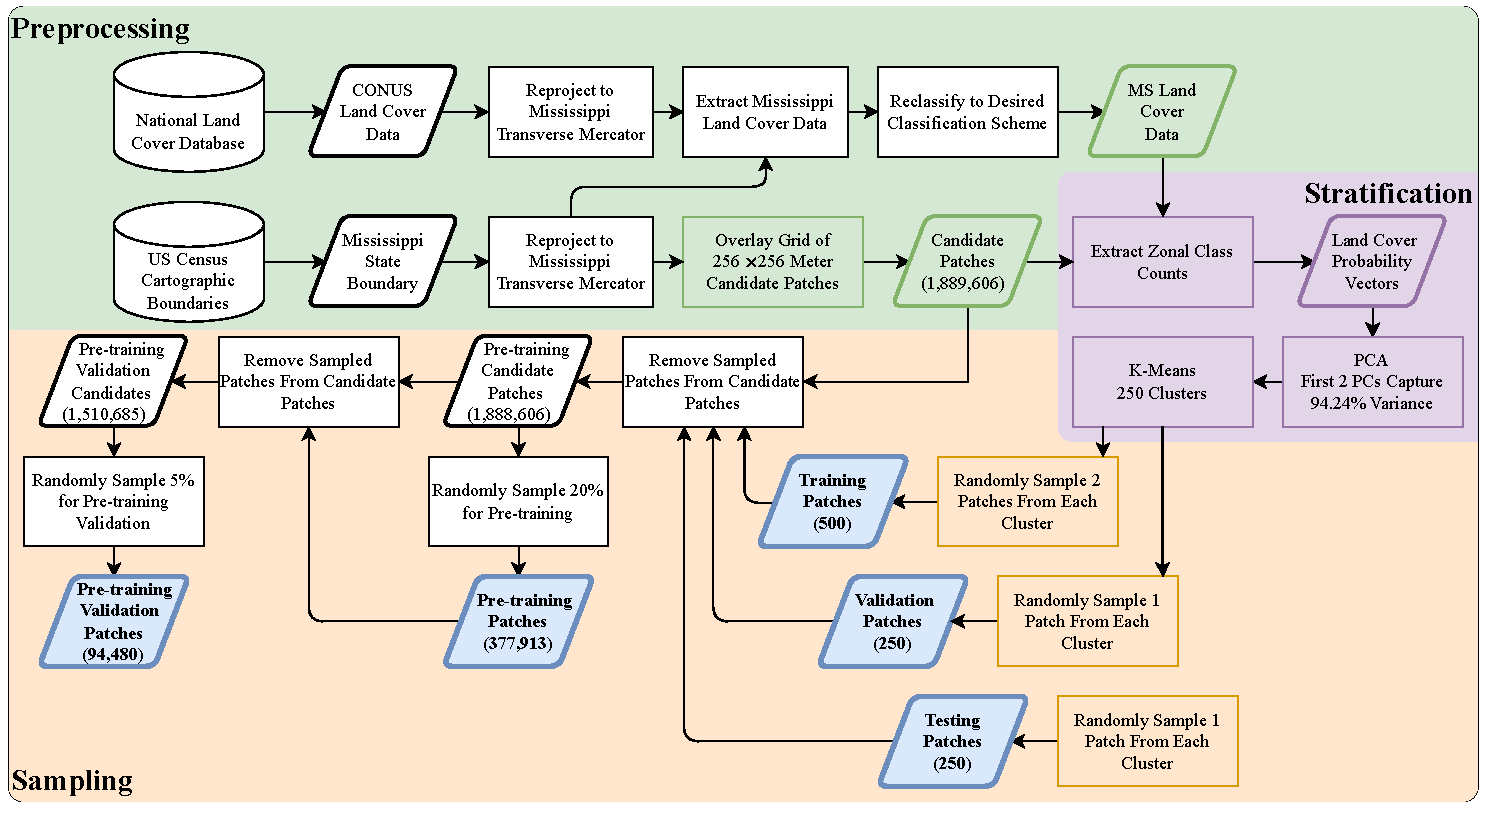
\includegraphics[width=\textwidth]{images/stratification_flowchart.drawio.pdf}
    \vspace{-0.75cm}
    \caption{Flowchart of the stratified sampling process for selecting data for model training and validation.}\label{fig:stratification_flowchart}
\end{figure}

\begin{figure}[ht]
    \centering
    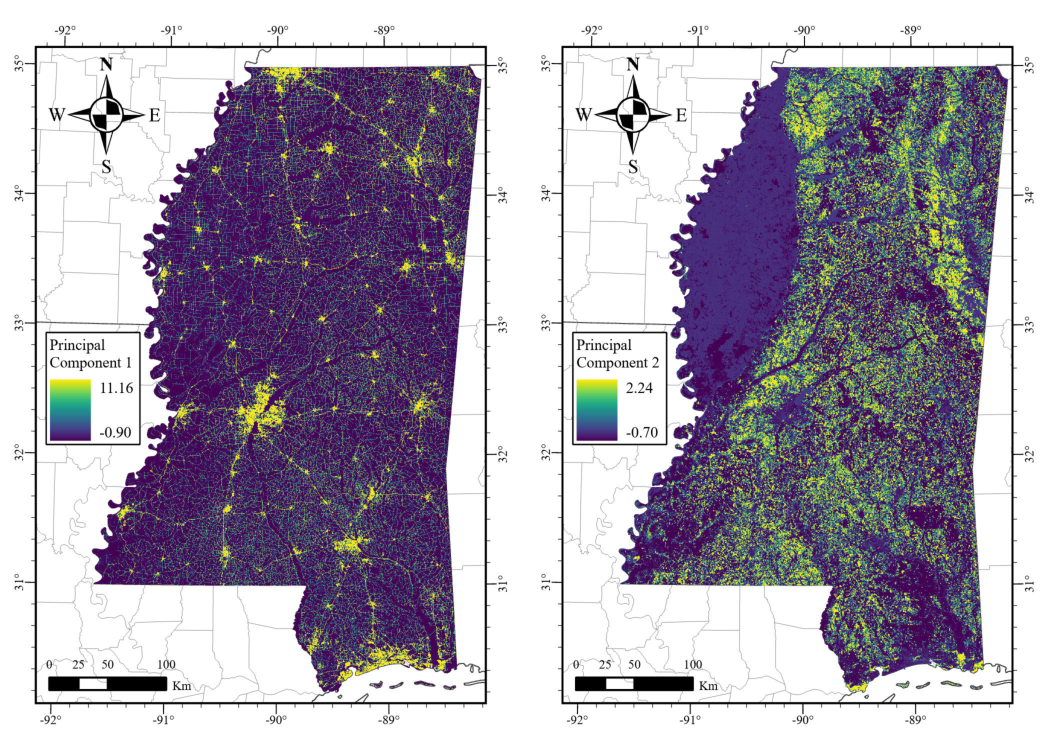
\includegraphics[width=\textwidth]{images/sampling/Mississippi_PCs.pdf}
    \caption{Principal components of NLCD relative frequencies per candidate tile.}\label{fig:ms_lc_pcs}
\end{figure}

\begin{figure}[ht]
    \centering
    
\includegraphics[width=0.8\textwidth]{images/sampling/clusters_250.png}
    \caption{Clusters from which samples are draw in principal component space.}\label{fig:clusters}
\end{figure}

Ensuring this strategy yields high-quality training data that is representative of the study area is crucial to the success 
However, a rigid evaluation of the stratification approach is not possible due to the lack of ground truth data for the study area.
One measure that can be taken to ensure the stratification is effective is to inspect the distribution of land cover classes across the splits.
Figure~\ref{fig:ms_lc_dist} shows that the distribution of land cover classes is consistent across the training, validation, and testing splits, which is ideal for ensuring that the model is exposed to a representative sample of the study area's land cover diversity.
One important note is that the distribution of land cover classes in the study area is highly imbalanced, with the majority of Mississippi's land cover being classified as forest, and a low density of urban and developed areas. 
To tackle this issue, other strategies often employ synthetic oversampling of minority classes to force the distribution of classes into a more balanced state~\cite{douzasImbalancedLearningLand2019, fonsecaImprovingImbalancedLand2021}.
Although the proposed approach to stratifying the data does not explicitly enforce such policies, comparing the land cover class distribution in the sampled tiles to the distribution across the entire state (as shown in Figure~\ref{fig:ms_lc_dist}) demonstrates that this sampling strategy achieves a similar outcome to such strategies.
Furthermore, this approach tends to avoid sampling tiles that are composed of a single land cover class. 
In the original NLCD data, 29.96\% of the tiles are composed of a single land cover class, while only 1.90\% of the sampled tiles are composed of a single land cover class.
This is promising, as heterogeneous tiles with a mixture of land cover classes convey information about the spatial organization of land cover classes.
Additionally, a visual inspection of the location of the sampled tiles in Figure~\ref{fig:sample_locations} shows that the tiles are distributed across the state of Mississippi without any apparent spatial bias.

\begin{figure}[H]
    \centering
    
\includegraphics[width=\textwidth]{images/sampling/split_distributions.png}
    \vspace{-0.75cm}
    \caption{Distribution of 2023 NLCD land cover classes across Mississippi: statewide distribution compared with training, validation, and test splits.}\label{fig:ms_lc_dist}
\end{figure}

\begin{figure}[H]
    \centering
    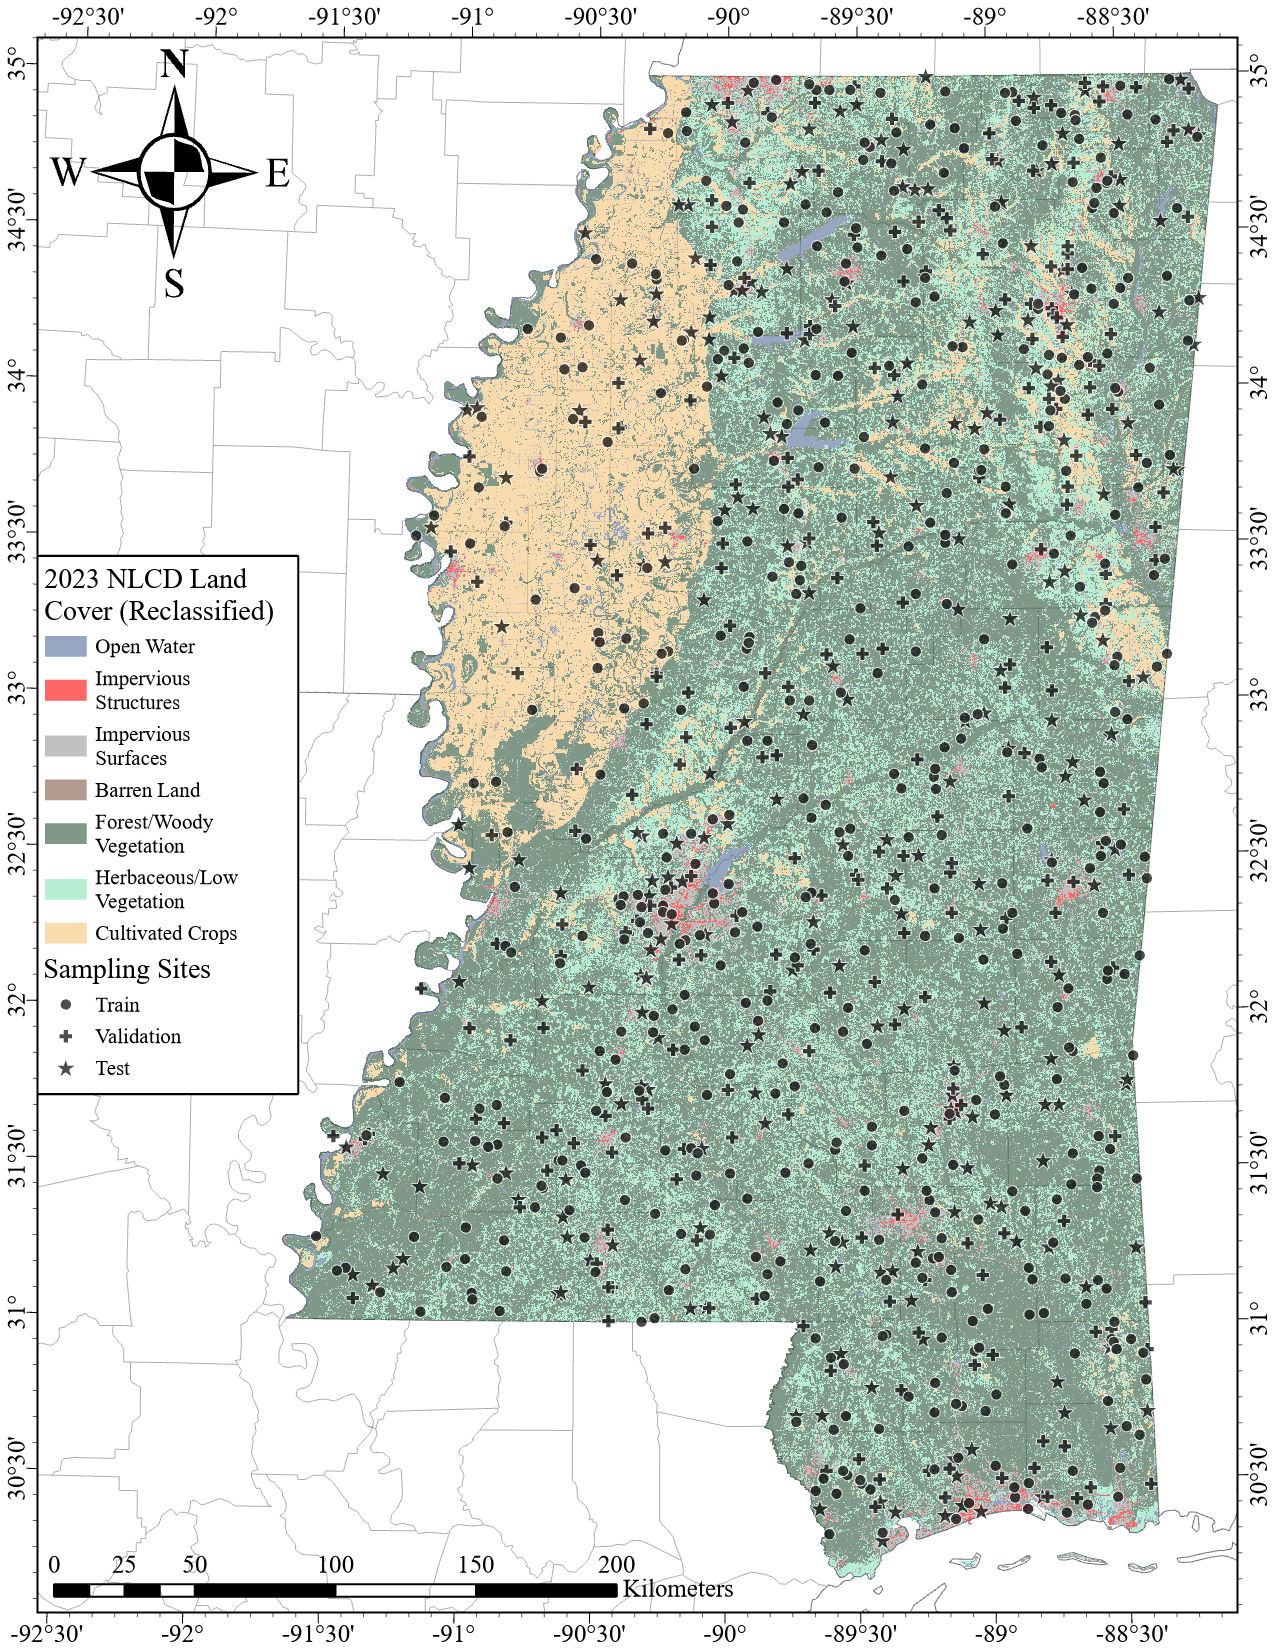
\includegraphics[height=0.9\textheight]{images/sampling/sampling_sites_map.pdf}
    % \vspace{-0.75cm}
    \caption{Sample locations for the Mississippi dataset.}\label{fig:sample_locations}
\end{figure}

\subsection{Attention U-NeXt semantic segmentation model}

The proposed Attention U-NeXt model is an encoder-decoder CNN model that builds upon the design of the Attention U-Net model~\cite{}